\formdesc{Modèle échantillonné du système à régler}

\underline{Boucle fermé hybride }

Parie analogique et numérique

\begin{center}
    \begin{tikzpicture}
        \begin{small} 
            \bXInput{E}
            \bXBloc[4]{D_A}{$D/A$}{E}
            \bXBloc[4]{Ga}{$G_a(s)$}{D_A}
            \bXBloc[4]{A_D}{$A/D$}{Ga}
            \bXOutput[4]{y}{A_D}

            \bXLink[$u(k)$]{E}{D_A}
            \bXLink[$u(t)$]{D_A}{Ga}
            \bXLink[$y(t)$]{Ga}{A_D}
            \bXLink[$y(k)$]{A_D}{y}
        \end{small}
    \end{tikzpicture}
\end{center}

Ce problème peut être résolu en utilisant le modèle échantillonné $H(z)$ dans les calculs dans le domaine en z.

\begin{center}
    \begin{tikzpicture}
        \begin{small} 
            \bXInput{E}
            \bXBloc[10]{H}{$H(z)$}{E}
            \bXOutput[10]{y}{H}

            \bXLink[$U(z)$]{E}{H}
            \bXLink[$Y(z)$]{H}{y}
        \end{small}
    \end{tikzpicture}
\end{center}


$H(z) = \cfrac{Y(z)}{U(u)}= \cfrac{z-1}{z} \cdot \mathcal{Z}\biggl\{ \mathcal{L}^-1\biggl( \cfrac{G_a(s)}{s}\biggr)\bigg|_{t = k\cdot h}\biggr\}$

Exemple :

\begin{enumerate}
    \item $\cfrac{G_a(s)}{s} = \cfrac{G_a(s)}{s(s-p_a)}$
    \item $\mathcal{L}^-1\biggl(\cfrac{G_a(s)}{s}\biggr) = \cfrac{ka}{-pa} \cdot 1-e^{p_a \cdot t}$ (Réponse indicielle)
    \item $\cfrac{ka}{-pa} \cdot 1-e^{p_a \cdot t}\bigg|_{t = k\cdot h} = \cfrac{ka}{-pa} \cdot 1-e^{p_a\cdot k\cdot h}$
    \item $\mathcal{Z}\biggl\{ \cfrac{ka}{-pa} \cdot 1-e^{p_a\cdot k\cdot h}  \biggr\} = \cfrac{ka}{-pa} \cfrac{z\cdot(1-e^{pa \cdot h})}{(z-1)\cdot(Z-e^{pa \cdot h})}$
    \item $\cfrac{z-1}{z} \mathcal{Z}\biggl\{...\biggr\} = \cfrac{ka}{-pa} \cfrac{1-e^{pa \cdot h}}{Z-e^{pa \cdot h}}$
\end{enumerate}

Donc les relations entre le plan s et Z sont : 

$p_n = e^{p_a\,h}$

$z = e^{s \, h}$

\underline{Propriétés du "modèle échantillonné"}
\begin{enumerate}
    \item pôles analogique se transforme selon $z = e^{s \, h}$
    \item Le gain  statique est préservé : $H(z = 1) = G_a(s = 0)$
    \item $H(z) $est linéaire en $G_a(s)$ : $G_{a1}(s) + G_{a2 }(s) \Leftrightarrow H_1(z) + H_2(z)$ Pas valable pour le produit 
    \item Un retard pur de N période coté analogique donne lieu à un facteur z dans la modèle échantillonné $e^{-H\,h}\Leftrightarrow z^N$
\end{enumerate}

\underline{Calcul du modèle échantillonné du système à régler}

le calcul se fait avec la réponse impulsionnelle.

$u[k] = \Delta[k]$ (Dirac numérique)

$\mathcal{L}\bigg(u(t) = \varepsilon(t) - \varepsilon(t-h)\bigg) = \cfrac{1}{s} - \cfrac{1}{s} \cdot e^{-h\,s} = U(s) $

Exemple sans retard : 

$u[k] = \{1,0,0,0\} \rightarrow y[k] = \{0,h,h,h\}$ (Intégrateur)

$y[k] =h \cdot \varepsilon[k-1] \rightarrow \mathcal{Z}(y) = H(z) = h \cdot z^{-1} \cfrac{z}{z-1} = \cfrac{h}{z-1} $

Exemple avec retard h/2 : 


$u[k] = \{1,0,0,0\} \rightarrow y[k] = \{0,h/2,h,h\}$ (Intégrateur)

$y[k] =h \cdot \varepsilon[k-2] + \cfrac{h}{2} \Delta[k-1]$

$\mathcal{Z}(y) = H(z) = h \cdot z^{-2} \cfrac{z}{z-1} + \cfrac{h}{2} \cdot z^{-1} = h\cfrac{1+\cfrac{1}{2}(z-1)}{z(z-1)} $


\underline{Avantages du modèle échantillonné}

\begin{itemize}
    \item Analyse et synthèse complètement en z
    \item Pas besoin de traiter le système hybride.
    \item Calculs exacts contrairement à l'inventaire des retards.
\end{itemize}

\underline{Correspondance entre le plan de s et le plan de z}

\begin{itemize}
    \item Le plan de z est "moins parlant" que le plan de s
    \item Beaucoup de caractéristiques, p.ex. taux d'amortissement sont définies en s
    \item Pour la synthèse par "placement de pôles", d'abord choisir les pôles en s et calculer les pôles en z correspondants
    \item Pour l'analyse, d'abord calculer les pôles en z, puis calculer les pôles en s correspondants en utilisant la fonction réciproque (log)
\end{itemize}

\underline{Avec ma calculatrice nulle}

$s = delta + j\omega$

$z = e^{s\,h} = e^{delta\,h + j\omega\,h} = 1\angle j\omega h $

$s = \cfrac{ln(z)}{h} = \cfrac{1}{h} \bigg(ln(|z|)+ln(e^{j\,arg(z)})\bigg) $

$=\cfrac{1}{h} \bigg(ln(|z|)+j\,arg(z)\bigg)$

\begin{figure}[H]
    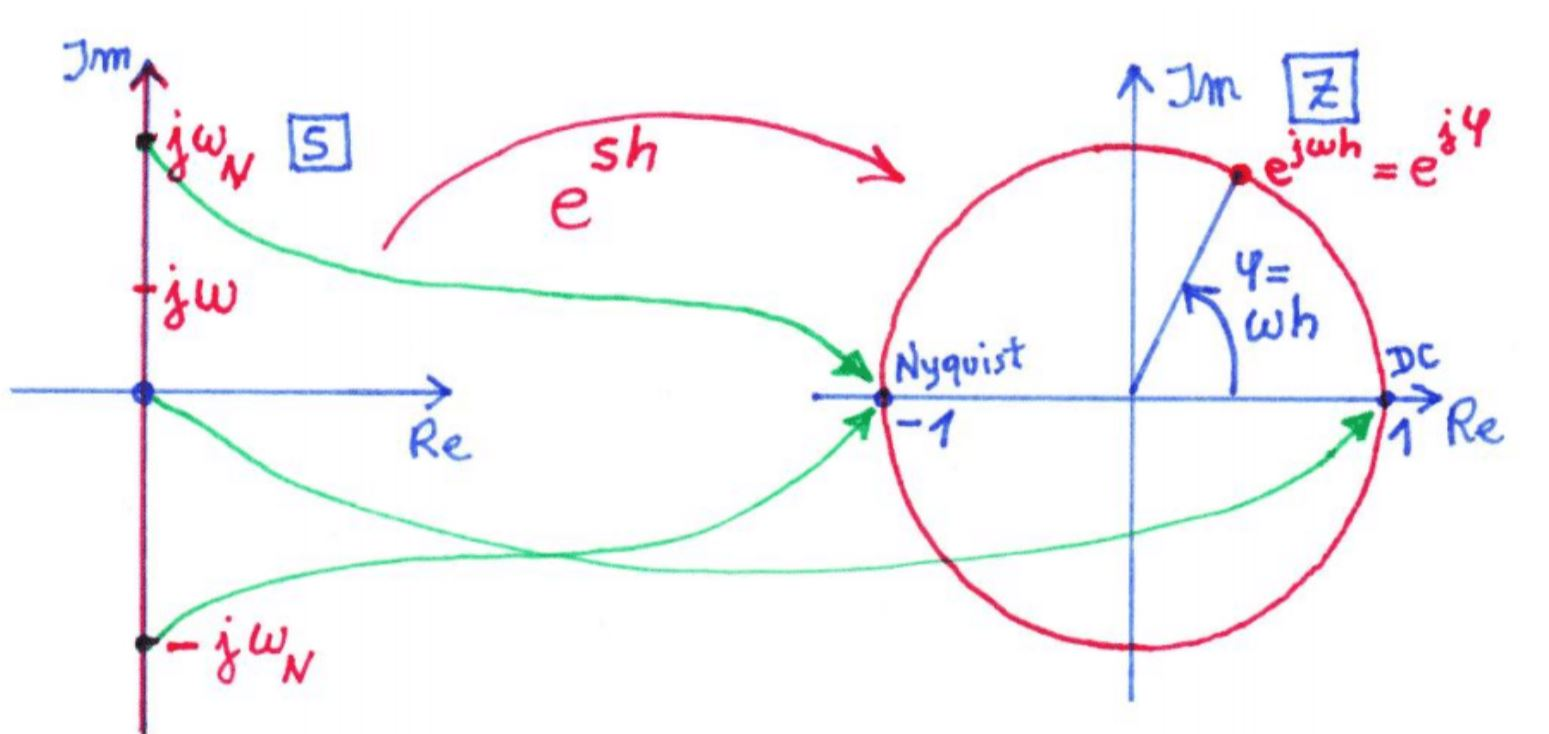
\includegraphics[width  = 0.48\textwidth]{img/ZtoS.JPG}
\end{figure}


